\begin{name}
	{\tenchude}
	{ĐỀ CỤM TRƯỜNG THPT-SỞ HẢI PHÒNG}
	{LỚP TOÁN THẦY PHÁT}
	{\lq\lq  Do what you can, with what you have, where you are.\rq\rq}
\end{name}

\Opensolutionfile{ansbook}[ans/ansb\currfilebase]
\caulc
\Opensolutionfile{ans}[ans/ans\currfilebase-Phan-I]
\begin{ex}%[Dự án 1]%[2H2H2-2]
	Trong không gian với hệ tọa độ $Oxyz$, cho ba điểm không thẳng hàng $A(-12;10;-2)$, $B(-4;6;9)$ và $E(6;-6;4)$. Để tứ giác $ABEF$ là hình bình hành thì tọa độ điểm $F$ là
	\choice
	{$(-14;10;-15)$}
	{$(-10;10;11)$}
	{$(-22;22;3)$}
	{\True $(-2;-2;-7)$}
	\loigiai{
		Ta có $\overrightarrow{AB}=(-4-(-12);6-10;9-(-2))=(8;-4;11)$.\\
		Gọi tọa độ điểm $F$ là $(x;y;z)$. Khi đó $\overrightarrow{FE}=(6-x;-6-y;4-z)$.\\
		Để tứ giác $ABEF$ là hình bình hành thì ta phải có $\overrightarrow{AB}=\overrightarrow{FE}$.
		$$\heva{&{8=6-x}\\&{-4=-6-y}\\&{11=4-z}}\Leftrightarrow \heva{&{x=6-8}\\&{y=-6+4}\\&{z=4-11}}\Leftrightarrow \heva{&x=-2\\&y=-2\\&z=-7.}$$
		Vậy tọa độ điểm $F$ là ($-2;-2;-7$).
	}
\end{ex}
\begin{ex}%[Dự án 1]%[2D1H5-1]
	\immini{
		Hàm số có đồ thị như hình vẽ là
		\choice
		{$y=\dfrac{-x}{x+1}$}
		{$y=\dfrac{-2x+1}{2x+1}$}
		{$y=\dfrac{-x+2}{x+1}$}
		{\True $y=\dfrac{-x+1}{x+1}$}}
	{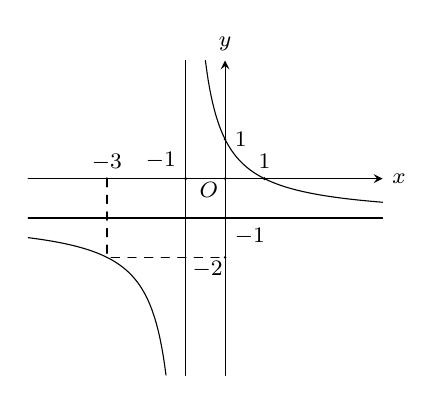
\begin{tikzpicture}[>=stealth,line join=round,line cap=round,font=\footnotesize,scale=0.5]
			\draw[->] (-5,0)--(4,0) node[right] {$x$};
			\draw[->] (0,-5)--(0,3) node[above] {$y$};
			\draw [smooth,domain=-0.5:4,samples=100]plot(\x,{(-\x+1)/(\x+1)});
			\draw [smooth,domain=-5:-1.5,samples=100]plot(\x,{(-\x+1)/(\x+1)});
			\draw (-5,-1)--(4,-1) (-1,-5)--(-1,3);
			\fill (0,0)node[shift={(-145:2.5mm)}]{\footnotesize{$O$}}circle(1pt) (1,0)node[above]{\footnotesize{$1$}}circle(1.2pt) (-1,0)node[above left]{\footnotesize{$-1$}}circle(1.2pt) (0,1)node[right]{\footnotesize{$1$}}circle(1pt)  (0,-1)node[below right]{\footnotesize{$-1$}}circle(1pt);
			\draw[dashed] (-3,0)|-(0,-2);
			\fill
			(-3,0) circle(1pt) node[shift=(90:0.2)]{$-3$}			
			(0,-2) circle(1pt) node[shift=(-145:0.27)]{$-2$};
	\end{tikzpicture}}
	\loigiai{Dựa vào hình vẽ, ta nhận thấy đồ thị hàm số nhận $x=-1$ và $y=-1$ làm hai đường tiệm cận. Đồng thời, đồ thị hàm số cắt trục $Ox$ và $Oy$ lần lượt tại $(1;0)$ và $(0;1)$ nên chỉ có hàm số $y=\dfrac{-x+1}{x+1}$ thỏa mãn.}
\end{ex}
\begin{ex}%[Dự án 1]%[1D2N3-2]
	Cho cấp số nhân $\left(u_{n}\right)$ biết $u_{3}=4$ và $u_{4}=8$. Công bội của cấp số nhân $(U_n)$ là
	\choice
	{$q=-4$}
	{\True $q=2$}
	{$q=\dfrac{1}{2}$}
	{$q=4$}
	\loigiai{
		Ta có $q=\dfrac{u_{4}}{u_{3}}=\dfrac{8}{4}=2$.
	}
\end{ex}
\begin{ex}%[Dự án 1]%[1D6H4-3]
	Tập nghiệm của bất phương trình $\log _{0{,}5}(x-1)>1$ là
	\choice
	{$\left(-\infty;-\dfrac{3}{2}\right)$}
	{$\left[1;\dfrac{3}{2}\right)$}
	{\True $\left(1;\dfrac{3}{2}\right)$}
	{$\left(\dfrac{3}{2};+\infty\right)$}
	\loigiai{
		Điều kiện xác định $x-1>0\Leftrightarrow x>1$.\\
		Ta có $\log _{0{,}5}(x-1)>1\Leftrightarrow x-1<(0{,}5)^{1}\Leftrightarrow x-1<0{,}5\Leftrightarrow x<1+0{,}5\Leftrightarrow x<\dfrac{3}{2}$\\
		Kết hợp nghiệm vừa tìm được với điều kiện $x>1$, ta có $\heva{&x>1\\&x<\dfrac{3}{2}}\Leftrightarrow 1<x<\dfrac{3}{2}$.\\
		Vậy tập nghiệm của bất phương trình là khoảng $\left(1;\dfrac{3}{2}\right)$.
	}
\end{ex}
\begin{ex}%[Dự án 1]%[2D1N3-1]
	\immini{
		Cho hàm số $y=f(x)$ có đồ thị như hình bên.
		Hàm số đã cho đạt giá trị nhỏ nhất trên đoạn $[-1;1]$ tại
		\choice[2]
		{\True $x=-1$}
		{$x=0$}
		{$x=-4$}
		{$x=1$}
	}{
		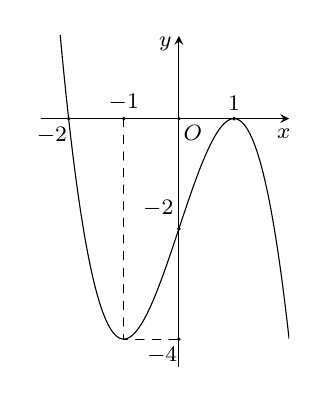
\begin{tikzpicture}[scale=0.7, font=\footnotesize, line join=round,
			line cap=round, >=stealth]
			\def \xmin{-2.5}
			\def \xmax{2}
			\def \ymin{-4.5}
			\def \ymax{1.5}
			\draw[->] (\xmin,0)--(\xmax,0) node[shift=(-110:0.2)] {$x$};
			\draw[->] (0,\ymin)--(0,\ymax) node[shift=(-150:0.2)] {$y$};
			\fill (0,0) circle(1pt) node[shift=(-45:0.25)]{$O$}
			(-2,0) circle(1pt) node[shift=(-135:0.3)]{$-2$}
			(1,0) circle(1pt) node[shift=(90:0.2)]{$1$}
			(-1,0) circle(1pt) node[shift=(90:0.2)]{$-1$}
			(0,-2) circle(1pt) node[shift=(135:0.37)]{$-2$}
			(0,-4) circle(1pt) node[shift=(-135:0.3)]{$-4$};
			\draw[dashed] (-1,0)|-(0,-4);
			\clip (\xmin,\ymin) rectangle (\xmax,\ymax);
			\draw[smooth,samples=100,domain=\xmin:\xmax] plot(\x,{-(\x)^3+3*(\x)-2});
		\end{tikzpicture}
	}
	\loigiai{
		Dựa vào đồ thị ta thấy hàm số đã cho đạt giá trị nhỏ nhất trên đoạn $[-1;1]$ tại điểm $x=-1$.
	}
\end{ex}
\begin{ex}%[Dự án 1]%[1H8H6-2]
	Cho hình chóp $S\cdot ABC$ có $SA\perp(ABC),SA=\dfrac{3a}{2}$, đáy $ABC$ là tam giác đều cạnh $a$. Số đo của góc nhị diện $[S,BC,A]$.
	\choice
	{$30^\circ$}
	{$90^\circ$}
	{$120^\circ$}
	{\True $60^\circ$}
	\loigiai{
\immini{
		Gọi $M$ là trung điểm $BC$.\\
		Vì tam giác $ABC$ đều cạnh $a$ nên $AM\perp BC$ $(1)$ và $AM=\dfrac{a\sqrt{3}}{2}$.\\
		Lại có $SA\perp(ABC)$ nên $SA\perp BC$, từ đó suy ra $SM\perp BC$ $(2)$.\\
		Từ $(1)$ và $(2)$ ta có $[S,BC,A]=\widehat{SMA}$.\\
		Tam giác $SAM$ vuông tại $A$, nên \\$\tan \widehat{SMA}=\dfrac{SA}{AM}=\dfrac{\dfrac{3a}{2}}{\dfrac{a\sqrt{3}}{2}}=\sqrt{3}\Rightarrow \widehat{SMA}=60^\circ$.
	}{
	\begin{tikzpicture}[scale=1, font=\footnotesize, line join=round, line cap=round, >=stealth]
		\path 
		(0,0) coordinate (A)
		(4,0) coordinate (C)
		(1.5,-1) coordinate (B)
		(0,3) coordinate (S)
		($(B)!.5!(C)$) coordinate (M)
		;
		\draw (B)--(C)--(S)--(A)--(B)--(S)--(M);
		\draw[dashed] (C)--(A)--(M);
		\foreach \d/\g in {A/180, C/0, B/-90, S/90,M/-45}
		\fill (\d) circle(1pt) + (\g:.3) node{$\d$};				
		\draw pic[draw,angle radius=2mm] {right angle = A--M--B};				
		\draw pic[draw,angle radius=5mm] {angle = S--M--A};			
		\end{tikzpicture}
	}
	}
\end{ex}
\begin{ex}%[Dự án 1]%[2D1N4-1]
	Cho hàm số $y=f(x)$ có bảng biến thiên như hình vẽ
	\begin{center}
		
\begin{tikzpicture}
			\tkzTabInit[nocadre=false,lgt=1.2,espcl=3,deltacl=0.5]
			{$x$/0.7,$f'(x)$/0.7,$f(x)$/2}
			{$-\infty$,$1$,$3$,$+\infty$}
			\tkzTabLine{,+,d,+,$0$,-,}
			\tkzTabVar{-/$-1$,+D-/$+\infty$/$-\infty$,+/$2$,-/$-\infty$}
		\end{tikzpicture}
	\end{center}
	Đồ thị hàm số $y=f(x)$ có tổng số đường tiệm cận đứng và ngang là
	\choice
	{\True $2$}
	{$0$}
	{$1$}
	{$3$}
	\loigiai{
		Từ bảng biến thiên, ta có $\lim\limits _{x\rightarrow 1^{+}}f(x)=-\infty$ nên đồ thị hàm số có đường tiệm cận đứng là $x=1$.\\
		Lại có $\lim\limits _{x\rightarrow-\infty}f(x)=-1$ nên đồ thị hàm số có đường tiệm cận ngang là $y=-1$.\\
		Vậy đồ thị hàm số $y=f(x)$ có tổng cộng $2$ đường tiệm cận đứng và ngang.
	}
\end{ex}
\begin{ex}%[Dự án 1]%[1D9H1-3]
	Hai khẩu pháo cao xạ cùng bắn độc lập với nhau vào một mục tiêu. Xác suất bắn trúng mục tiêu của hai khẩu pháo cao xạ lần lượt là $\dfrac{1}{4}$ và $\dfrac{1}{3}$. Xác xuất để mục tiêu bị bắn trúng đạn là
	\choice
	{\True $\dfrac{1}{2}$}
	{$\dfrac{7}{12}$}
	{$\dfrac{5}{12}$}
	{$\dfrac{1}{4}$}
	\loigiai{
		Gọi $A$ là biến cố \lq\lq Xạ thủ 1 bắn trúng mục tiêu\rq\rq.\\
		$B$ là biến cố \lq\lq Xạ thủ 2 bắn trúng mục tiêu\rq\rq.\\
		$M$ là biến cố \lq\lq Mục tiêu bị bắn trúng\rq\rq.\\
		Theo giả thiết ta có $\mathrm{P}(A)=\dfrac{1}{4}\Rightarrow \mathrm{P}\left(\overline{A}\right)=1-\dfrac{1}{4}=\dfrac{3}{4}$.\\
		Lại có $\mathrm{P}(B)=\dfrac{1}{3}\Rightarrow \mathrm{P}\left(\overline{B}\right)=1-\dfrac{1}{3}=\dfrac{2}{3}$.\\
		Ta có $\overline{M}=\overline{A}\cap \overline{B}$.\\
		Vì $A$ và $B$ là hai biến cố độc lập nên $\overline{A}$ và $\overline{B}$ cũng là hai biến cố độc lập.\\		
		Do đó $\mathrm{P}\left(\overline{M}\right)=\mathrm{P}\left(\overline{A}\right)\cdot \mathrm{P}\left(\overline{B}\right)=\dfrac{3}{4}\cdot \dfrac{2}{3}=\dfrac{1}{2}$.\\
		Vậy $\mathrm{P}(M)=1-\mathrm{P}\left(\overline{M}\right)=\dfrac{1}{2}$.
	}
\end{ex}
\begin{ex}%[Dự án 1]%[1D1N5-3]
	Phương trình $\sin x=-1$ có nghiệm là
	\choice
	{$x=\dfrac{\pi}{2}+k2\pi$, $k\in \mathbb{Z}$}
	{$x=\pi+k2\pi$, $k\in \mathbb{Z}$}
	{$x=k\pi$, $k\in \mathbb{Z}$}
	{\True $x=-\dfrac{\pi}{2}+k2\pi$, $k\in \mathbb{Z}$}
	\loigiai{
		Ta có $\sin x=-1\Leftrightarrow x=-\dfrac{\pi}{2}+k2\pi$, $k\in \mathbb{Z}$.
	}
\end{ex}
\begin{ex}%[Dự án 1]%[1D5H1-3]
	Khảo sát thu nhập theo tháng của người lao động ở một công ty thu được mẫu số liệu ghép nhóm như sau
	\begin{center}
		\begin{tabular}{|c|c|c|c|c|c|}
			\hline
			Thu nhập (triệu đồng) & $[5;8)$ & $[8;11)$ & $[11;14)$ & $[14;17)$ & $[17;20)$ \\
			\hline
			Số người & $30$ & $55$ & $45$ & $30$ & $20$ \\
			\hline
		\end{tabular}
	\end{center}
	Thu nhập trung bình của người lao động của công ty là
	\choice
	{$10{,}5$}
	{\True $11{,}75$}
	{$12{,}5$}
	{$11$}
	\loigiai{
		\begin{center}
			\begin{tabular}{|c|c|c|c|c|c|}
				\hline
				Thu nhập (triệu đồng) & $[5;8)$ & $[8;11)$ & $[11;14)$ & $[14;17)$ & $[17;20)$ \\
				\hline
				Số người & $30$ & $55$ & $45$ & $30$ & $20$ \\
				\hline
				Giá trị đại diện & $6{,}5$ & $9{,}5$ & $12{,}5$ & $15{,}5$ & $18{,}5$ \\
				\hline
			\end{tabular}
		\end{center}
		Thu nhập trung bình của người lao động công ty là
		\[\overline{x}=\dfrac{6{,}5\cdot 30+9{,}5\cdot 55+12{,}5\cdot 45+15{,}5\cdot 30+18{,}5\cdot 20}{30+55+45+30+20}\approx 11{,}75\cdot \]
	}
\end{ex}
\begin{ex}%[Dự án 1]%[2D1N2-2]
	Cho hàm số $y=f(x)$ có bảng biến thiên như hình vẽ
	\begin{center}
		
\begin{tikzpicture}
			\tkzTabInit[nocadre=false, lgt=1.2, espcl=3, deltacl=0.5]
			{$x$/0.7,$f'(x)$/0.7,$f(x)$/2}
			{$-\infty$,$0$,$3$,$+\infty$}
			\tkzTabLine{+,$0$,-,$0$,+,}
			\tkzTabVar{-/$-\infty$,+/$2$,-/$-3$,+/$+\infty$}
		\end{tikzpicture}
	\end{center}
	Hàm số $f(x)$ đạt cực tiểu tại điểm	
	\choice
	{$y=0$}
	{$x=-4$}
	{$y=-4$}
	{\True $x=3$}
	\loigiai{Từ bảng biến thiên, suy ra $f(x)$ đạt cực tiểu tại điểm $x=3$.		
	}
\end{ex}
\begin{ex}%[Dự án 1]%[2H2H2-2]
	Trong không gian $Oxyz$, cho điểm $A(1;0;1)$. Tọa độ điểm $C$ thỏa mãn $\overrightarrow{AC}=(3;3;0)$ là
	\choice
	{$C(2;3;1)$}
	{$C(3;3;0)$}
	{$C(-3;-3;-1)$}
	{\True $C(4;3;1)$}
	\loigiai{
		Giả sử $C(x;y;z)\Rightarrow \overrightarrow{AC}=(x-1;y;z-1)$.\\
		Do $\overrightarrow{AC}=(3;3;0)\Leftrightarrow\heva{&x-1=3\\&y=3\\&z-1=0}\Leftrightarrow\heva{&x=4\\&y=3\\&z=1.}$\\
		Vậy $C(4;3;1)$.
	}
\end{ex}
\Closesolutionfile{ans}
\cauds
\Opensolutionfile{ans}[ans/ans\currfilebase-Phan-II]
\begin{ex}%[Dự án 1]%[2H5V2-7]
	Cho hình vuông $ABCD$ có cạnh bằng $4$. Lấy $H$, $K$ lần lượt trên các cạnh $AB$, $AD$ sao cho $BH=3HA$, $AK=3KD$. Trên đường thẳng vuông góc với mặt phẳng $(ABCD)$ tại $H$ lấy điểm $S$ sao cho $\widehat{SBH}=30^\circ$.			
	\choiceTF
	{Thể tích của khối chóp $S.ABC$ bằng $\dfrac{16\sqrt{3}}{3}$}
	{\True Khoảng cách giữa $AB$ và $SD$ bằng $\dfrac{4\sqrt{57}}{19}$}
	{\True $SH=\sqrt{3}$}
	{\True Gọi $E$ là giao điểm của $CH$ và $BK$, cosin của góc giữa hai đường thẳng $SE$ và $BC$ bằng $\dfrac{m}{n\sqrt{39}}$ với $m\in \mathbb{Z}$; $n\in \mathbb{N}^{*}$; $\dfrac{m}{n}$ là phân số tối giản. Giá trị của $T=2m-n=31$}
	\loigiai{
		\begin{center}
			\begin{tikzpicture}[scale=1.3, font=\footnotesize, line join=round, line cap=round, >=stealth]
				\path 
				(0,0) coordinate (A)
				(4,0) coordinate (D)
				(-1.5,-1) coordinate (B)
				($(B)+(D)-(A)$) coordinate (C)
				($(B)!3/4!(A)$) coordinate (H)
				($(A)!3/4!(D)$) coordinate (K)
				($(H)+(D)-(A)$) coordinate (F)
				($(H)+(0,3)$) coordinate (S)
				($(S)!2/3!(F)$) coordinate (N)
				($(H)!1.3!(S)$) coordinate (z)
				($(H)!1.3!(F)$) coordinate (y)
				($(A)!1.3!(B)$) coordinate (x)
				(intersection of K--B and C--H) coordinate (E)
				;
				\draw (S)--(B)--(C)--(D)--(S)--(C) (S)--(F);
				\draw[dashed] (S)--(A)--(D) (A)--(B) (S)--(H)--(C) (B)--(K) (H)--(F) (S)--(E) (H)--(N);
				\draw [->] (S)--(z);
				\draw [->] (F)--(y);
				\draw [->] (B)--(x);
				\foreach \d/\g in {A/45, C/-45, B/135,D/45, S/135,H/-90,E/-90,F/-45,N/-90,K/145}
				\fill (\d) circle(1pt) + (\g:.25) node{$\d$};
				\foreach \d/\g in {x/130,y/90,z/0}
				\fill (\d) + (\g:.25) node{$\d$};
				\foreach \x/\y/\z in {S/H/A} \draw pic[draw,angle radius=2mm] {right angle= \x--\y--\z};							
				\draw pic[draw,angle radius=5mm] {angle = A--B--S};			
			\end{tikzpicture}
		\end{center}		
		\begin{itemchoice}			
			\itemch
			Ta có $V_{S.ABCD}=\dfrac{1}{3}SH\cdot S_{ABCD}$.\\
			$S_{ABCD}=4^{2}=16$, $HB=\dfrac{3}{4}AB=3$, $\tan 30^\circ=\dfrac{SH}{HB}\Rightarrow SH=3\cdot \tan 30^\circ=\sqrt{3}$.\\
			Suy ra $V_{S.ABCD}=\dfrac{1}{3}\cdot \sqrt{3}\cdot 16=\dfrac{16\sqrt{3}}{3}$ mà $V_{S.ABC}=\dfrac{1}{2}V_{S.ABCD}=\dfrac{8\sqrt{3}}{3}$.
			\itemch
			Dựng $HF\perp CD$ tại $F$ và $HN\perp SF$ tại $N$.\\
			Ta có $AB\parallel (SCD)$ nên $\mathrm{d}(AB,SD)=\mathrm{d}\left(AB,\left(SCD\right)\right)=\mathrm{d}\left(H,\left(SCD\right)\right)=HN$.\\
			Xét tam giác $SHF$ vuông tại $H$, ta có 
			\begin{eqnarray*}
				&&\dfrac{1}{HS^{2}}+\dfrac{1}{HF^{2}}=\dfrac{1}{HN^{2}}\\
				&\Leftrightarrow& \dfrac{1}{(\sqrt{3})^{2}}+\dfrac{1}{4^{2}}=\dfrac{1}{HN^{2}}\\
				&\Rightarrow& HN=\dfrac{4\sqrt{57}}{19}.
			\end{eqnarray*}
			Vậy $\mathrm{d}(AB,SD)=\dfrac{4\sqrt{57}}{19}$.
			\itemch
			Ta có $SH=\sqrt{3}$
			\itemch
			Đặt hệ trục $Oxyz$ như hình vẽ.\\
			Ta có
			$H(0;0;0)$, $S\left(0;0;\sqrt{3}\right)$, $B(3;0;0)$, $C(3;4;0)$, $K(-1;3;0)$.\\
			Mà $E=CH\cap BK$ với $CH\colon \heva{&x=3t\\&y=4t\\&z=0}$ và $BK\colon \heva{&x=3-4t'\\&y=3t'\\&z=0}$ 
			nên $\heva{&3t=3-4t'\\&4t=3t'}\Leftrightarrow\heva{&t=\dfrac{9}{25}\\&t'=\dfrac{12}{25}}$.\\			
			Suy ra
			$E\left(\dfrac{27}{25};\dfrac{36}{25};0\right)$.\\
			Do đó
			$\overrightarrow{SE}=\left(\dfrac{27}{25};\dfrac{36}{25};-\sqrt{3}\right)$, $\overrightarrow{BC}=(0;4;0)$.\\
			Khi đó
			$$\cos (SE,BC)=\left|\cos \left(\overrightarrow{SE},\overrightarrow{BC}\right)\right|=\dfrac{\left|\overrightarrow{SE}\cdot \overrightarrow{BC}\right|}{\left|\overrightarrow{SE}\right|\cdot \left|\overrightarrow{BC}\right|}=\dfrac{\dfrac{144}{25}}{\dfrac{2\sqrt{39}}{5}\cdot 4}=\dfrac{18}{5\sqrt{39}.}$$
			Suy ra $m=18$, $n=5$.\\
			Vậy $T=2m-n=2\cdot 18-5=31$.
		\end{itemchoice}
	}
\end{ex}
\begin{ex}%[Dự án 1]%[2H2H2-6]
	\immini{
	Trong không gian, xét hệ tọa độ $Oxyz$ có gốc $O$ trùng với vị trí một giàn khoan trên biển, mặt phẳng $(Oxy)$ trùng với mặt biển (được gọi là mặt phẳng) với tia $Ox$ hướng về phía nam, tia $Oy$ hướng về phía đông, tia $Oz$ hướng thẳng lên trời (tham khảo hình vẽ). Đơn vị đo trong không gian $Oxyz$ lấy theo kilômét. Một chiếc radar đặt tại $O$ có phạm vi theo dõi $30$ km. Một chiếc tàu thám hiểm tại vị trí $A$ ở độ sâu $10$ km so với mặt nước biển, cách $O25$\,km về phía nam và $15$\,km về phía tây. Một tàu đánh cá tại vị trí $B(-20;15;0)$.
}{
		\begin{tikzpicture}[line join = round, line cap=round,>=stealth,font=\footnotesize,scale=.55]
			\definecolor{xanhdatroi}{RGB}{30,144,255}
			\tikzset{icon-cot/.pic={
					\path
					(0,0)coordinate (A)
					($(A)+(0,8)$)coordinate (B)
					($(B)+(-2,-1)$)coordinate (C)
					($(A)+(C)-(B)$)coordinate (D)
					($(C)!(A)!(D)$)	 coordinate (A1)
					($2*(A1)-(A)+(0,1)$)coordinate (E)
					($(B)+(E)-(A)$) coordinate (F)
					;
					
					\draw (A)--(B)--(C)--(D)--cycle
					(D)--(E)--(F)--(C);
					\foreach \x/\y in {0/0.1,0.1/0.2,0.2/0.3,0.3/0.4,0.4/0.5,0.5/0.6,0.6/0.7,0.7/0.8,0.8/0.9,0.9/1}
					\draw
					($(A)!\x!(B)$)--($(D)!\y!(C)$)
					($(D)!\x!(C)$)--($(A)!\y!(B)$)
					($(E)!\x!(F)$)--($(D)!\y!(C)$)
					($(D)!\x!(C)$)--($(E)!\y!(F)$)
					($(A)!\x!(B)$)--($(E)!\y!(F)$)
					($(E)!\x!(F)$)--($(A)!\y!(B)$)
					(B)--(F) (A)--(E);
			}}
			
			\fill[bottom color=blue!80!green!15!black, top color=blue!20!green!20, middle color=blue!80!green]
			(-5,-5) rectangle (6,2);
			\fill[inner color=xanhdatroi, outer color=xanhdatroi!50]
			(-5,5) rectangle (6,2);
			
			%%%%%%%%%%%%%%%%%%%%%%%%%%%%%%%%%%%%
			\path
			(0.75,-1.2)  pic[scale=0.15]{icon-cot}
			(0.75,-1.5)  pic[scale=0.15]{icon-cot}
			(1.8,-1.2) pic[scale=0.15]{icon-cot}
			(1.8,-1.5) pic[scale=0.15]{icon-cot}
			(2.8,-1.2) pic[scale=0.15]{icon-cot}
			(2.8,-1.5) pic[scale=0.15]{icon-cot}
			;
			%%%%%%%%%%%%%%%%%%%%%%%%%%%%%%%%
			\draw[fill=orange!10,scale=1,yshift=-1.25cm,xshift=-0.3cm,opacity=0.2,decorate, decoration={snake, amplitude=0.4mm, segment length=2mm},scale=1.2]
			(-1.5,0.5)--(0.5,-0.5)--(4.5,-0.5) --($(-1.5,0.5)+(4.5,-1)-(0.5,-1)$)--cycle
			;
			%%%%%%%%%%%%%%%%%%%%%%%%%%%%%%%%
			\draw[fill=orange,scale=1]
			(-1.5,0.5)--(0.5,-0.5)--(4.5,-0.5) --($(-1.5,0.5)+(4.5,-1)-(0.5,-1)$)--cycle
			;
			%%%%%%%%%%%%%%%%%%%%%%%%%%%%%%%%
			\path
			(0.75,0) pic[scale=0.15]{icon-cot}
			(0.75,0.2) pic[scale=0.15]{icon-cot}
			(1.8,0) pic[scale=0.15]{icon-cot}
			(1.8,0.2) pic[scale=0.15]{icon-cot}
			(2.8,0) pic[scale=0.15]{icon-cot}
			(2.8,0.2) pic[scale=0.15]{icon-cot}
			;
			\begin{scope}
				\draw[->,line width=2pt,red] (0,0)--(4,-2)node[above]{$y$};
				\draw[->,line width=2pt,red] (0,0)--(-4,0)node[above]{$x$};
				\draw[->,line width=2pt,red] (0,0)--(0,4)node[above]{$z$};
				\fill (0,0) circle(1.5pt) node[above left]{$O$};
			\end{scope}
			%%%%%%%%%%%%%%%%%%%%%%%%%%%%%%%%%%%%
		\end{tikzpicture}
	}
	\choiceTF
	{\True Một chiếc tàu của cảnh sát biển đang tuần tra di chuyển đến vị trí $C$ cách $O$ một khoảng $15$\,km về phía nam. Để radar phát hiện ra thì tàu cảnh sát biển cần di chuyển về phía đông cách $O$ tối đa $15\sqrt{3}$\,km}
	{\True Radar phát hiện ra tàu đánh cá tại vị trí $B$}
	{Khoảng cách từ chiếc tàu thám hiểm đến radar bằng $3\sqrt{58}$\,km}
	{\True Radar không phát hiện được tàu thám hiểm đặt tại vị trí $A$}
	\loigiai{
		\begin{itemchoice}	
			\itemch
			Gọi $x$ (km), $x>0$ là khoảng cách từ tàu cảnh sát biển cách radar $O$ về phía đông.\\
			Khi đó toạ độ của tàu cảnh sát biển là $C(15;x;0)$. Ta có $OC=\sqrt{15^{2}+x^{2}+0^{2}}=\sqrt{x^{2}+225}$.\\
			Để radar phát hiện được tàu cảnh sát biển thì $OC\leq 30$\,km.\\
			Suy ra $\sqrt{x^{2}+225}\leq 30\Leftrightarrow x^{2}+225\leq 900\Leftrightarrow x^{2}\leq 675\Leftrightarrow x\leq 15\sqrt{3}$\,km.\\
			Vậy tàu cảnh sát biển cần di chuyển về phía đông cách $O$ tối đa $15\sqrt{3}$\,km.
			\itemch
			Ta có $OB=\sqrt{(-20)^{2}+15^{2}+0^{2}}=25$\,(km) $<30$\,(km) nên radar phát hiện ra tàu đánh cá tại vị trí $B$.
			\itemch
			Một chiếc tàu thám hiểm tại vị trí $A$ ở độ sâu $10$ km so với mặt nước biển, cách $O$ một khoảng $25$\,km về phía nam và $15$ km về phía tây nên ta có tọa độ tàu thám hiểm là điểm tọa độ điểm $A(25;-15;-10)$. Khi đó khoảng cách từ chiếc tàu thám hiểm đến radar bằng $$OA=\sqrt{25^{2}+(-15)^{2}+(-10)^{2}}=5\sqrt{38}\,(\mathrm{km}).$$
			\itemch
			Ta thấy $OA=5\sqrt{38}$\,(km) $\approx 30{,}82$\,(km,) mà phạm vi theo dõi của radar là $30$\,km nên radar không phát hiện được tàu thám hiểm đặt tại vị trí $A$.
			
	\end{itemchoice}}
\end{ex}
\begin{ex}%[Dự án 1]%[2D1V5-7]
	Cho hàm số $f(x)=\dfrac{2x^{2}-5x+9}{x-5}$.
	\choiceTF
	{\True Đồ thị hàm số cắt trục tung tại điểm có tung độ bằng $-\dfrac{9}{5}$}
	{Hàm số nghịch biến trên khoảng ($1;9$)}
	{Có đúng một điểm trên đồ thị cách đều hai trục tọa độ}
	{Đồ thị hàm số có tiệm cận đứng là $y=5$}
	\loigiai{
		\begin{itemchoice}	
			\itemch
			Với $x=0\Rightarrow f(0)=-\dfrac{9}{5}$.\\
			Vậy đồ thị hàm số cắt trục tung tại điểm có tung độ bằng $-\dfrac{9}{5}$.
			\itemch
			Tập xác định của hàm số là $\mathbb{R}\backslash\{5\}$ suy ra hàm số đã cho không xác định $\forall x\in(1;9)$.
			\itemch
			Gọi $M\left(x_{0};y_{0}\right)$ thuộc đồ thị hàm số (điều kiện $x_{0}\neq 5$)\\
			Vì điểm $M\left(x_{0};y_{0}\right)$ trên đồ thị cách đều hai trục tọa độ nên $y_{0}=\pm x_{0}$
			\begin{itemize}
				\item \textbf{Trường hợp 1}.
				\allowdisplaybreaks
				\begin{eqnarray*}
					y_{0}=x_{0}
					&\Leftrightarrow& \dfrac{2x_{0}{}^{2}-5x_{0}+9}{x_{0}-5}=x_{0}\\
					&\Leftrightarrow& 2x_{0}{}^{2}-5x_{0}+9=x_{0}{}^{2}-5x_{0}\\
					&\Leftrightarrow& x_{0}{}^{2}+9=0 \text{ (phương trình vô nghiệm).}
				\end{eqnarray*}
				\item \textbf{Trường hợp 2}.
				\allowdisplaybreaks
				\begin{eqnarray*}
					y_{0}=-x_{0}
					&\Leftrightarrow& \dfrac{2x_{0}{}^{2}-5x_{0}+9}{x_{0}-5}=-x_{0}\\
					&\Leftrightarrow& 2x_{0}{}^{2}-5x_{0}+9=-x_{0}{}^{2}+5x_{0}\\
					&\Leftrightarrow& 3x_{0}^{2}-10x_{0}+9=0 \text{ (phương trình vô nghiệm).}
				\end{eqnarray*}
			\end{itemize}			
			Vậy không có điểm nào trên đồ thị cách đều hai trục tọa độ
			\itemch
			Đồ thị hàm số có tiệm cận đứng là $x=5$.
		\end{itemchoice}
	}
\end{ex}
\begin{ex}%[Dự án 1]%[1D1V5-5]
	Cho phương trình $\cos \left(4x-\dfrac{3\pi}{8}\right)=-1$.
	\choiceTF
	{\True $x=\dfrac{11\pi}{32}$ là một nghiệm của phương trình đã cho}
	{\True Tất cả nghiệm của phương trình đã cho được biểu diễn bởi $4$ điểm trên đường tròn lượng giác}
	{Tổng nghiệm dương nhỏ nhất và nghiệm âm lớn nhất của phương trình bằng $\dfrac{3\pi}{4}$}
	{Tổng các nghiệm trên khoảng $\left(\dfrac{\pi}{4};\dfrac{19\pi}{2}\right)$ của phương trình đã cho là $\dfrac{6\,061\pi}{32}$}
	\loigiai{
		\begin{itemchoice}	
			\itemch Thay $x=\dfrac{11\pi}{32}$ vào phương trình, ta được $\cos \left(4\cdot \dfrac{11\pi}{32}-\dfrac{3\pi}{8}\right)=\cos (\pi)=-1$.\\
			Vậy $x=\dfrac{11\pi}{32}$ là một nghiệm của phương trình đã cho.
			\itemch
			Ta có 
			\allowdisplaybreaks
			\begin{eqnarray*}
				&&\cos \left(4x-\dfrac{3\pi}{8}\right)=-1\\
				&\Leftrightarrow& 4x-\dfrac{3\pi}{8}=\pi+k2\pi\\
				&\Leftrightarrow& 4x=\dfrac{11\pi}{8}+k2\pi\\
				&\Leftrightarrow& x=\dfrac{11\pi}{32}+\dfrac{k\pi}{2}(k\in \mathbb{Z})
			\end{eqnarray*}
			Áp dụng công thức nghiệm $x=\alpha+\dfrac{k2\pi}{n}$ với $n$ là số điểm biểu diễn trên đường tròn lượng giác.\\
			Ta có $x=\dfrac{11\pi}{32}+\dfrac{k\pi}{2}=\dfrac{11\pi}{32}+\dfrac{k2\pi}{4}$.\\
			Suy ra $n=4$.\\
			Vậy tất cả nghiệm của phương trình đã cho được biểu diễn bởi $4$ điểm trên đường tròn lượng giác.
			\itemch
			Xét $x=\dfrac{11\pi}{32}+\dfrac{k\pi}{2}>0\Leftrightarrow \dfrac{k\pi}{2}>-\dfrac{11\pi}{32}\Leftrightarrow k>-\dfrac{11}{16}$.\\
			Mà $k\in \mathbb{Z}$, suy ra, nghiệm dương nhỏ nhất ứng với $k=0$.\\ 
			Nghiệm dương nhỏ nhất là $\dfrac{11\pi}{32}+\dfrac{0\cdot \pi}{2}=\dfrac{11\pi}{32}$.\\
			Xét $x=\dfrac{11\pi}{32}+\dfrac{k\pi}{2}<0\Leftrightarrow \dfrac{k\pi}{2}<-\dfrac{11\pi}{32}\Leftrightarrow k<-\dfrac{11}{16}$.\\
			Mà $k\in \mathbb{Z}$, suy ra, nghiệm âm lớn nhất ứng với $k=-1$.\\
			Nghiệm âm lớn nhất là $\dfrac{11\pi}{32}+\dfrac{(-1)\cdot \pi}{2}=-\dfrac{5\pi}{32}$.\\
			Tổng nghiệm dương nhỏ nhất và nghiệm âm lớn nhất của phương trình bằng $\dfrac{11\pi}{32}-\dfrac{5\pi}{32}=\dfrac{3\pi}{16}$.
			\itemch
			Do $x\in\left(\dfrac{\pi}{4};\dfrac{19\pi}{2}\right)$, ta có 
			\allowdisplaybreaks
			\begin{eqnarray*}
				\dfrac{\pi}{4}<x<\dfrac{19\pi}{2}
				&\Leftrightarrow& \dfrac{\pi}{4}<\dfrac{11\pi}{32}+\dfrac{k\pi}{2}<\dfrac{19\pi}{2}\\
				&\Leftrightarrow& \dfrac{1}{4}<\dfrac{11}{32}+\dfrac{k}{2}<\dfrac{19}{2}\\
				&\Leftrightarrow&-\dfrac{3}{32}<\dfrac{k}{2}<\dfrac{293}{32}\\
				&\Leftrightarrow&-\dfrac{3}{16}<k<\dfrac{293}{16}.
			\end{eqnarray*}
			Do $k\in \mathbb{Z}$, suy ra $k\in\{0;1;2;\ldots;17;18\}$.\\
			Thay các giá trị của $k$ vào $x=\dfrac{11\pi}{32}+\dfrac{k\pi}{2}$ ta được tập hợp các nghiệm trên khoảng $\left(\dfrac{\pi}{4};\dfrac{19\pi}{2}\right)$, ta được
			$$x\in\left\{\dfrac{11\pi}{32};\dfrac{11\pi}{32}+\dfrac{\pi}{2};\dfrac{11\pi}{32}+\dfrac{2\pi}{2};\ldots;\dfrac{11\pi}{32}+\dfrac{17\pi}{2};\dfrac{11\pi}{32}+\dfrac{18\pi}{2}\right\}.$$
			Vậy tổng các nghiệm  $\sum_{k=0}^{18}\left(\dfrac{11\pi}{32}+\dfrac{k\pi}{2}\right)=\dfrac{2945\pi}{32}$.		
		\end{itemchoice}
	}
\end{ex}
\Closesolutionfile{ans}
\caukq
\Opensolutionfile{ans}[ans/ans\currfilebase-Phan-III]
\begin{ex}%[Dự án 1]%[1H8V5-4]
	Cho hình chóp $S\cdot ABCD$ có đáy $ABCD$ là hình thoi cạnh 1, góc $\widehat{BAD}=60^\circ$. Tam giác $SAB$ vuông cân tại $S$ và nằm trong mặt phẳng vuông góc với đáy. Biết khoảng cách từ $AB$ đến $SC$ bằng $\dfrac{\sqrt{a}}{b}$ ($a$; $b\in \mathbb{Z}^*$) ($\dfrac{a}{b}$ là phân số tối giản). Tổng $a+b$ bằng
	\par
	\shortans[0]{7}
	\loigiai{
\immini{Vì $\widehat{BAD}=60^\circ$ nên $\triangle ABC$ là tam giác đều cạnh bằng $1$.\\
		Gọi $I$ là trung điểm của $AB$.\\
		$\triangle ABD$ là tam giác đều nên $DI\perp AB$.\\
		Vì tam giác $SAB$ vuông cân tại $S$ và nằm trong mặt phẳng vuông góc với đáy nên $SI\perp(ABCD)$.\\
		Gọi $H$ là chân đường vuông góc kẻ từ $I$ đến $SD$.\\
		$\heva{&AB\perp SI\\&AB\perp DI}\Rightarrow AB\perp(SDI)\Rightarrow AB\perp IH$.\\
		Mà $AB\parallel CD$ do đó $IH\perp CD$.\\
		Lại có $IH\perp SD$ suy ra $IH\perp(SCD)$.\\
		Ta có $AB\parallel CD$ nên $AB\parallel (SCD)$.}{
	\begin{tikzpicture}[scale=1.3, font=\footnotesize, line join=round, line cap=round, >=stealth]
	\path 
	(0,0) coordinate (A)
	(4,0) coordinate (D)
	(-1.5,-1) coordinate (B)
	($(B)+(D)-(A)$) coordinate (C)
	($(B)!.5!(A)$) coordinate (I)
	($(C)!.5!(A)$) coordinate (O)
	($(I)+(0,3)$) coordinate (S)
	($(S)!1/3!(D)$) coordinate (H)			
	;
	\draw (S)--(B)--(C)--(D)--(S)--(C);
	\draw[dashed] (S)--(A)--(D) (S)--(I)--(D) (B)--(A)--(C) (I)--(H) (B)--(D);
	\foreach \d/\g in {A/45, C/-45, B/135,D/45, S/90,H/60,I/135,O/-90}
	\fill (\d) circle(1pt) + (\g:.25) node{$\d$};
	\foreach \x/\y/\z in {S/I/A,D/I/B,D/O/C,S/H/I} \draw pic[draw,angle radius=2mm] {right angle= \x--\y--\z};									
\end{tikzpicture}		
		}\noindent
		Khi đó $\mathrm{d}(AB,SC)=\mathrm{d}(AB,(SCD))=\mathrm{d}(I,(SCD))=IH$.\\
		Ta có $ID=\dfrac{\sqrt{3}}{2}$ và $SI=\dfrac{1}{2}AB=\dfrac{1}{2}$ suy ra $IH=\sqrt{\dfrac{SI^{2}\cdot ID^{2}}{SI^{2}+ID^{2}}}=\sqrt{\dfrac{\left(\dfrac{1}{2}\right)^{2}\cdot\left(\dfrac{\sqrt{3}}{2}\right)^{2}}{\left(\dfrac{1}{2}\right)^{2}+\left(\dfrac{\sqrt{3}}{2}\right)^{2}}}=\dfrac{\sqrt{3}}{4}$.\\
		Suy ra $a=3$ và $b=4$.\\
		Vậy $a+b=7$.
	}
\end{ex}
\begin{ex}%[Dự án 1]%[2D1V3-6]
	Một doanh nghiệp sản xuất độc quyền một loại sản phẩm. Giả sử khi sản xuất và bán hết $x$ sản phẩm ($0<x\leq 2500$), tổng số tiền doanh nghiệp thu được là $f(x)=2006x-x^{2}$ (đơn vị: nghìn đồng) và tổng chi phí là $g(x)=x^{2}+1438x-1209$ (đơn vị: nghìn đồng). Giả sử mức thuế phụ thu trên một đơn vị sản phẩm bán được là $t$ (nghìn đồng) ($0<t<320$). Để nhà nước nhận được số tiền thuế phụ thu lớn nhất và doanh nghiệp cũng nhận được lợi nhuận lớn nhất theo mức thuế phụ thu đó thì giá trị của $t$ bằng bao nhiêu nghìn đồng.
	\par
	\shortans[0]{284}
	\loigiai{
		Gọi $h(x)$ là lợi nhuận của doanh nghiệp khi bán $x$ sản phẩm với mức thuế $t$.\\
		Ta có $h(x)=f(x)-g(x)-tx=\left(2006x-x^{2}\right)-\left(x^{2}+1438x-1209\right)-tx$.\\
		Suy ra $h(x)=-2x^{2}+(568-t)x+1209$, ta có $h'(x)=-4x+(568-t)\Rightarrow h'(x)=0\Leftrightarrow x=\dfrac{568-t}{4}$.\\
		Vì $h(x)$ là hàm bậc hai có $a<0$ nên suy ra $\max h(x)=\pi\left(\dfrac{568-t}{4}\right)$.\\
		Số tiền thuế nhà nước thu được để doanh nghiệp cũng nhận được lợi nhuận lớn nhất là $T(t)$:\\
		$T(t)=tx=t\left(\dfrac{568-t}{4}\right)=\dfrac{1}{4}t(568-t)\leq \dfrac{1}{4}\left(\dfrac{t+568-t}{2}\right)^{2}=20\,164$.\\
		Dấu \lq\lq $=$\rq\rq\,xẩy ra khi và chỉ khi $t=568-t\Leftrightarrow t=284$ (thỏa mãn điều kiện $0<t<320$).\\
		Suy ra, $\max T(t)=20\,164$ khi $t=284$.\\
		Vậy giá trị của thuế phụ thu cần tìm là $t=284$ (nghìn đồng).
	}
\end{ex}
\begin{ex}%[Dự án 1]%[1D2V3-8]
	Trong năm đầu tiên đi làm, anh Huy nhận được lương là $10$ triệu đồng mỗi tháng. Cứ hết một năm, anh Huy lại được tăng lương, mỗi tháng năm sau tăng $12\%$ so với mỗi tháng năm trước. Kể từ năm thứ $2$ mỗi khi lĩnh lương anh Huy đều cất đi phần tăng lương so với năm ngay trước để tiết kiệm mua ô tô. Hỏi tính từ khi đi làm sau ít nhất bao nhiêu năm thì anh Huy mua được ô tô giá $500$ triệu biết rằng anh Huy được gia đình hỗ trợ $32\%$ giá trị chiếc xe?
	\par
	\shortans[0]{13}
	\loigiai{
		Số tiền mà anh Huy phải trả để mua xe ô tô là $500\cdot 0{,}68=340$ (triệu đồng).\\
		Tổng tiền lương năm đầu tiên anh Huy nhận được là $T_{1}=10\cdot 12=120$ (triệu đồng).\\
		Số tiền tiết kiệm được của anh Huy sau năm thứ hai là $T_{2}=120\cdot 1{,}02-120=120\cdot 0{,}12$ (triệu đồng).\\
		Số tiền tiết kiệm được của anh Huy sau năm thứ ba là $T_{3}=120\cdot 1{,}12^{2}-120\cdot 1{,}12=120\cdot 1{,}12\cdot 0{,}12$ (triệu đồng).\\
		Số tiền tiết kiệm được của anh Huy sau năm thứ $n$ là $T_{n}=120\cdot 1{,}12^{n-2}\cdot 0{,}12$ (triệu đồng).\\
		Tổng số tiền tiết kiệm của anh Huy sau $n$ năm là
		\allowdisplaybreaks
		\begin{eqnarray*}
			T&=&T_{2}+T_{3}+\cdots+T_{n}\\
			&=&120\cdot 0{,}12\left(1+1{,}12+1{,}12^{2}+\cdots+1{,}12^{n-2}\right)\\
			&=&120\cdot 0{,}12\cdot \dfrac{1{,}12^{n-1}-1}{1{,}12-1}\\
			&=&120\cdot\left(1{,}12^{n-1}-1\right) \text{(triệu đồng)}.
		\end{eqnarray*}
		Để anh Huy đủ tiền mua xe thì
		$$T\geq 340\Leftrightarrow 120\cdot\left(1{,}12^{n-1}-1\right)\geq 340\Leftrightarrow n-1\geq \log _{1{,}12}\left(\dfrac{23}{6}\right)\Leftrightarrow n\geq 12{,}8.$$
		Vậy tính từ khi đi làm, phải ít nhất $13$ năm thì anh Huy mới đủ tiền mua ô tô.
	}
\end{ex}
\begin{ex}%[Dự án 1]%[2H2V2-6]
	Hai chiếc flycam được điều khiển cùng bay lên tại một địa điểm. Sau một thời gian bay, chiếc flycam thứ nhất cách điểm xuất phát về phía Bắc $20$ (m) và về phía Tây $10$ (m), đồng thời cách mặt đất $0,7$ (m). chiếc flycam thứ hai cách điểm xuất phát về phía Nam $30$ (m) và về phía Đông $25$ (m), đồng thời cách mặt đất $1$ (m). Trên mặt đất người ta xác định một vị trí sao cho tổng khoảng cách từ đó đến hai chiếc flycam ngắn nhất. Khoảng cách (m) từ điểm xuất phát đến vị trí vừa xác định được bằng bao nhiêu \textit{(kết quả làm tròn đến hàng phần trăm)}?
	\par
	\shortans[0]{$4,45$}
	\loigiai{
	Chọn hệ trục tọa độ $Oxyz$, đơn vị trên mỗi trục tọa độ là $1$ (m).\\
	$O(0;0;0)$ là điểm xuất phát.
	\immini{
	Trục $Ox$ là hướng Bắc.\\
	Trục $Oy$ là hướng Tây.\\
	Trục $Oz$ hướng lên trên.\\
	Mặt đất là mặt phẳng $(Oxy)$.\\
	Theo giả thiết, sau một thời gian bay, chiếc flycam thứ nhất có tọa độ là $A(20;10;0,7)$, chiếc flycam thứ hai có toạ độ là $B(-30;-25;1)$.\\
	Gọi $A'$ là điểm đối xứng với $A$ qua mặt phẳng $(Oxy)$.\\
	Ta có $A'(20;10;-0,7)$.\\
	Gọi $C$ là điểm trên mặt đất thì $C(x;y;0)$.\\
	Khi đó, ta có $CA+CB=CA'+CB\geq A'B$.
}{
\begin{tikzpicture}[scale=0.7, font=\footnotesize, line join=round, line cap=round, >=stealth]
			\path
			(0,0) coordinate (O)
			(-2,-2) coordinate (A)
			(3,-2) coordinate (H)
			(5,0) coordinate (B)
			(3,1) coordinate (M)
			(0,3) coordinate (C)
			%%
			($(O)!-0.7!(H)$) coordinate (K)
			($(O)!-0.7!(A)$) coordinate (A')
			($(O)!-0.7!(B)$) coordinate (B')
			($(K)+(0,2.5)$) coordinate (M')
			;
			\draw[->] (-4.5,0)--(6,0) node[below]{$x$};
			%	\draw[->] (2,2)--(-2.5,-2.5) node[left]{$y$};
			\draw[->] (2,2)--(-2.5,-2.5) node[left]{$y$};
			\draw[->] (0,0)--(0,4.5) node[left]{$z$};
			\draw[dashed] (M)--(H)--(A) (O)--(H)--(B) (O)--(K) (B')--(K)--(A') (K)--(M');
			
			\draw[fill=black] (O) circle (.05) +(-90:.3)node{\footnotesize $O$};
			\draw[fill=black] (M) circle (.05) +(0:.3)node{\footnotesize $A$};
			\draw[fill=black] (M') circle (.05) +(0:.3)node{\footnotesize $B$};
			\end{tikzpicture}}
\noindent
Dấu \lq\lq$=$\rq\rq\, xảy ra khi $A'$, $C$, $B$ thẳng hàng.\\
Mặt khác $\overrightarrow{A'C}=(x-20;y-10;0{,}7)$; $\overrightarrow{A'B}=(-50;-35;1{,}7)$.\\
Điều kiện để $3$ điểm $A'$ $C$, $B$ thẳng hàng là tồn tại $k\in \mathbb{R}$ sao cho
$$\overrightarrow{A'C}=k\overrightarrow{A'B}
\Leftrightarrow\heva{&x-20=-50k\\&y-10=-35k\\&0{,}7=1{,}7k}\Leftrightarrow\heva{&k=\dfrac{7}{17}\\&x=-\dfrac{10}{17}\\&y=-\dfrac{75}{17}.}$$
Suy ra $C\left(-\dfrac{10}{17};-\dfrac{75}{17};0\right)$ là vị trí trên mặt đất có tổng khoảng cách từ đó đến hai chiếc flycam ngắn nhất.\\
Khi đó khoảng cách từ điểm xuất phát $O$ đến $C$ là 
$OC=\sqrt{\left(-\dfrac{10}{17}\right)^{2}+\left(-\dfrac{75}{17}\right)^{2}+0^{2}}\approx 4{,}45$ (m). 
	}
\end{ex}

\begin{ex}%[Dự án 1]%[0D0V2-6]
	Một đa giác đều có $20$ đỉnh, tất cả các cạnh của đa giác sơnn màu xanh và tất cả các đường chéo của đa giác đó sơn màu đỏ. Gọi $X$ là tập hợp tất cả các tam giác có ba đỉnh là các đỉnh của đa giác đều trên. Người ta chọn ngẫu nhiêu từ $X$ một tam giác. Xác suất để chọn được tam giác có ba cạnh cùng màu là $\dfrac{a}{b}$ ($a\in \mathbb{N}$, $ b\in \mathbb{N}^*$; $\dfrac{a}{b}$ là phân số tối giản). Khi đó $a+b$ bằng
	\par
	\shortans[0]{$97$}
	\loigiai{
		Ta có $n(X)=C_{20}^{3}=1\,140$.\\
		Dễ thấy không thể có tam giác nào có $3$ cạnh đều là cạnh của đa giác đều ban đầu.\\
		Gọi $A_{k}$ là biến cố \lq\lq tam giác được chọn có $k$ cạnh màu xanh\rq\rq.
		\begin{itemize}
			\item Trường hợp 1: tam giác có $2$ cạnh màu xanh.\\
			Để được tam giác như thế thì $2$ cạnh màu xanh là $2$ cạnh của đa giác, khi đó ta cần chọn $3$ đỉnh liên tiếp của đa giác. Do đó $n\left(A_{2}\right)=20$.\\
			\item Trường hợp 2: tam giác có $1$ cạnh màu xanh.\\
			Để được tam giác như thế thì ta cần chọn $2$ đỉnh liên tiếp của đa giác, đỉnh còn lại của tam giác không kề với $2$ đỉnh kia.\\
			Chọn $2$ đỉnh liên tiếp, có $20$ cách chọn.\\
			Chọn đỉnh còn lại, bỏ $2$ đỉnh đã chọn và $2$ đỉnh kề với $2$ đỉnh đó, có $16$ cách chọn.\\
			Do đó $n\left(A_{1}\right)=20\cdot 16=320$.\\
			Suy ra $n\left(A_{0}\right)=1\,140-20-320=800$.\\
			Xác suất cần tìm là $\mathrm{P}\left(A_{0}\right)=\dfrac{800}{1\,140}=\dfrac{40}{57}$ hay $a=40$, $b=57$.\\
		\end{itemize}		
		Vậy $a+b=40+57=97$.
	}
\end{ex}
\begin{ex}%[Dự án 1]%[1D6V2-5]
	Nguồn âm đẳng hướng đặt tại điểm $O$ có công suất truyền âm không đổi. Mức cường độ âm tại điểm $M$ cách điểm $O$ một khoảng $R$ được tính bởi công thức $L_{M}=\log \dfrac{k}{R^{2}}$ (Ben) với $k$ là hằng số. Biết điểm $O$ thuộc đoạn thẳng $AB$ và mức cường độ âm tại $A$ và $B$ lần lượt là $L_{A}=5$ (Ben) và $L_{B}=7$ (Ben). Tính mức cường độ âm (Ben) tại trung điểm $AB$ \textit{(kết quả làm tròn đến hàng phần trăm)}
	\par\shortans[0]{5,69}
	\loigiai{
		Gọi $H$ là trung điểm $AB$.Ta có\\
		$L_{A}=\log \dfrac{k}{OA^{2}}=5\Leftrightarrow OA^{2}=\dfrac{k}{10^{5}}$.\\
		$L_{B}=\log \dfrac{k}{OB^{2}}=7\Leftrightarrow OB^{2}=\dfrac{k}{10^{7}}$.
		Ta có
		\begin{itemize}
			\item \textbf{Trường hợp 1}. Điểm $O$ nằm gần điểm $A$,ta có $OH=\dfrac{OB-OA}{2}$.
			\begin{center}
				\begin{tikzpicture}[scale=1, font=\footnotesize, line join=round, line cap=round, >=stealth]
					\path 
					(0,0) coordinate (A)
					(2,0) coordinate (O)
					(4,0) coordinate (H)
					(8,0) coordinate (B)
					;			
					\draw (A)--(B);
					\foreach \d/\g in {A/180,B/0,O/90,H/90}
					\fill (\d) circle(1pt) + (\g:.25) node{$\d$};											
				\end{tikzpicture}
			\end{center}
			Ta có
			\allowdisplaybreaks
			\begin{eqnarray*}
				L_{H}&=&\log \dfrac{k}{OH^{2}}\\
				&=&\log \dfrac{4k}{OB^{2}-2OA\cdot OB+OA^{2}}\\
				&=&\log \dfrac{4k}{\dfrac{k}{10^{7}}-2\cdot \dfrac{k}{10^{6}}+\dfrac{k}{10^{5}}}\\
				&=&\log \dfrac{4}{\dfrac{1}{10^{7}}-2\cdot \dfrac{1}{10^{6}}+\dfrac{1}{10^{5}}}\\
				&\approx& 5{,}69
			\end{eqnarray*}
			\item \textbf{Trường hợp 2}. Điểm $O$ nằm gần điểm $B$, ta có $OH=\dfrac{OA-OB}{2}$.
			\begin{center}
				\begin{tikzpicture}[scale=1, font=\footnotesize, line join=round, line cap=round, >=stealth]
					\path 
					(0,0) coordinate (A)
					(6,0) coordinate (O)
					(4,0) coordinate (H)
					(8,0) coordinate (B)
					;			
					\draw (A)--(B);
					\foreach \d/\g in {A/180,B/0,O/90,H/90}
					\fill (\d) circle(1pt) + (\g:.25) node{$\d$};											
				\end{tikzpicture}
			\end{center}
			Ta có
			\allowdisplaybreaks
			\begin{eqnarray*}
				L_{H}&=&\log \dfrac{k}{OH^{2}}\\
				&=&\log \dfrac{4k}{OA^{2}-2OA\cdot OB+OB^{2}}\\
				&=&\log \dfrac{4k}{\dfrac{k}{10^{5}}-2\cdot \dfrac{k}{10^{6}}+\dfrac{k}{10^{7}}}\\
				&=&\log \dfrac{4}{\dfrac{1}{10^{5}}-2\cdot \dfrac{1}{10^{6}}+\dfrac{1}{10^{7}}}\\
				&\approx& 5{,}69
			\end{eqnarray*}
		\end{itemize}	
	}
\end{ex}
\Closesolutionfile{ans}
\Closesolutionfile{ansbook}
% \begin{indapan}
% 	{ans/ans\currfilebase}
% \end{indapan}